%%%%%%%%%%%%%%%%%%%%%%%%%%%%%%%%%%%%%%%%%%%%%%%%%%%%%%%%%%%%
% 1.6 FIELD THEORY
% The Composition of Advanced Mathematics
%%%%%%%%%%%%%%%%%%%%%%%%%%%%%%%%%%%%%%%%%%%%%%%%%%%%%%%%%%%%

\section{Field Theory}
\label{sec:field-theory}

\prerequisite{
Functions from \cref{sec:functions}, methods of proof from
\cref{sec:methods-of-proof}, elementary algebra from
\cref{sec:elementary-algebra}, linear algebra from
\cref{sec:linear-algebra}, abstract algebra from
\cref{sec:abstract-algebra}, group theory from
\cref{sec:group-theory}, and ring theory from
\cref{sec:ring-theory}.
}

\learningobjectives{
By the end of this section, the reader should be able to:
\begin{itemize}
    \item verify whether an algebraic system is a field;
    \item distinguish fields from rings, integral domains, and division rings;
    \item work with finite fields of prime order;
    \item determine the characteristic of a field;
    \item recognize the prime subfield of a field;
    \item define and work with field extensions;
    \item distinguish algebraic and transcendental elements;
    \item find minimal polynomials in elementary cases;
    \item interpret the degree of a field extension;
    \item use the Tower Law;
    \item construct simple extensions;
    \item construct fields using polynomial quotient rings;
    \item recognize splitting fields;
    \item understand algebraic closures;
    \item distinguish finite, algebraic, and transcendental extensions;
    \item understand the role of finite fields;
    \item recognize how field extensions prepare the foundation for Galois theory.
\end{itemize}
}

%%%%%%%%%%%%%%%%%%%%%%%%%%%%%%%%%%%%%%%%%%%%%%%%%%%%%%%%%%%%
\subsection{Why Fields?}
\label{subsec:why-fields}
%%%%%%%%%%%%%%%%%%%%%%%%%%%%%%%%%%%%%%%%%%%%%%%%%%%%%%%%%%%%

Elementary algebra frequently assumes that nonzero quantities can be divided.

For example, from

\[ ax=b,\qquad a\neq0, \]

we solve by writing

\[ x=a^{-1}b=\frac{b}{a}. \]

This step is not available in an arbitrary ring because a nonzero element
need not possess a multiplicative inverse.

Fields are precisely the commutative algebraic systems in which division by
every nonzero element is possible.

\begin{conceptbox}
A field is a commutative ring in which every nonzero element has a
multiplicative inverse.

Fields provide the natural scalar systems for linear algebra and the natural
setting for much of polynomial algebra.
\end{conceptbox}

%%%%%%%%%%%%%%%%%%%%%%%%%%%%%%%%%%%%%%%%%%%%%%%%%%%%%%%%%%%%
\subsection{Definition of a Field}
\label{subsec:definition-field}
%%%%%%%%%%%%%%%%%%%%%%%%%%%%%%%%%%%%%%%%%%%%%%%%%%%%%%%%%%%%

\begin{definitionbox}{Field}
A \emph{field} is a commutative ring \(F\) with
\[ 1\neq0 \]
such that every nonzero \(a\in F\) has a multiplicative inverse
\[ a^{-1}\in F. \]
\end{definitionbox}

Equivalently,

\[ (F,+) \]

is an abelian group and

\[ (F\setminus\{0\},\cdot) \]

is also an abelian group, with multiplication distributing over addition.

%%%%%%%%%%%%%%%%%%%%%%%%%%%%%%%%%%%%%%%%%%%%%%%%%%%%%%%%%%%%
\subsection{The Two Group Structures of a Field}
\label{subsec:field-two-groups}
%%%%%%%%%%%%%%%%%%%%%%%%%%%%%%%%%%%%%%%%%%%%%%%%%%%%%%%%%%%%

A field contains two closely related group structures.

\begin{center}
\begin{tikzpicture}[
    node distance=13mm and 22mm,
    box/.style={draw,rounded corners,align=center,inner sep=5pt},
    >=stealth
]
\node[box] (F) {Field \(F\)};
\node[box,below left=of F] (add) {\((F,+)\)\\abelian group};
\node[box,below right=of F] (mult) {\((F\setminus\{0\},\cdot)\)\\abelian group};
\node[box,below=18mm of F] (dist) {Distributive laws};

\draw[->] (F)--(add);
\draw[->] (F)--(mult);
\draw[->] (add)--(dist);
\draw[->] (mult)--(dist);
\end{tikzpicture}
\end{center}

The element \(0\) is excluded from the multiplicative group because \(0\)
cannot have a multiplicative inverse in a nontrivial field.

%%%%%%%%%%%%%%%%%%%%%%%%%%%%%%%%%%%%%%%%%%%%%%%%%%%%%%%%%%%%
\subsection{Standard Examples of Fields}
\label{subsec:standard-fields}
%%%%%%%%%%%%%%%%%%%%%%%%%%%%%%%%%%%%%%%%%%%%%%%%%%%%%%%%%%%%

The most familiar fields are

\[ \Q,\qquad\R,\qquad\C. \]

The rational numbers form a field because every nonzero rational number

\[ \frac{a}{b} \]

has inverse

\[ \frac{b}{a}. \]

The real and complex numbers similarly support addition, subtraction,
multiplication, and division by nonzero elements.

%%%%%%%%%%%%%%%%%%%%%%%%%%%%%%%%%%%%%%%%%%%%%%%%%%%%%%%%%%%%
\subsection{The Integers Are Not a Field}
\label{subsec:integers-not-field}
%%%%%%%%%%%%%%%%%%%%%%%%%%%%%%%%%%%%%%%%%%%%%%%%%%%%%%%%%%%%

The integers form an integral domain but not a field.

For example,

\[ 2\in\Z, \]

but its multiplicative inverse

\[ \frac12 \]

does not belong to \(\Z\).

Therefore,

\[ \Z \]

is not a field.

This illustrates the structural difference between integral domains and
fields.

%%%%%%%%%%%%%%%%%%%%%%%%%%%%%%%%%%%%%%%%%%%%%%%%%%%%%%%%%%%%
\subsection{The Field Hierarchy}
\label{subsec:field-hierarchy}
%%%%%%%%%%%%%%%%%%%%%%%%%%%%%%%%%%%%%%%%%%%%%%%%%%%%%%%%%%%%

The major ring structures introduced so far fit into the hierarchy

\begin{center}
\begin{tikzpicture}[
    node distance=10mm,
    box/.style={draw,rounded corners,align=center,inner sep=5pt,font=\small},
    >=stealth
]
\node[box] (ring) {Ring};
\node[box,below=of ring] (comm) {Commutative ring};
\node[box,below=of comm] (domain) {Integral domain};
\node[box,below=of domain] (field) {Field};

\draw[->,thick] (ring)--node[right]{commutative multiplication}(comm);
\draw[->,thick] (comm)--node[right]{no zero divisors}(domain);
\draw[->,thick] (domain)--node[right]{nonzero inverses}(field);
\end{tikzpicture}
\end{center}

Every field is an integral domain.

Not every integral domain is a field.

%%%%%%%%%%%%%%%%%%%%%%%%%%%%%%%%%%%%%%%%%%%%%%%%%%%%%%%%%%%%
\subsection{Every Field Is an Integral Domain}
\label{subsec:field-integral-domain}
%%%%%%%%%%%%%%%%%%%%%%%%%%%%%%%%%%%%%%%%%%%%%%%%%%%%%%%%%%%%

\begin{theorem}
Every field is an integral domain.
\end{theorem}

\begin{proof}
Let \(F\) be a field and suppose

\[ ab=0. \]

If \(a=0\), the conclusion already holds.

Suppose \(a\neq0\). Since \(F\) is a field, \(a^{-1}\) exists.

Multiplying by \(a^{-1}\),

\[ a^{-1}(ab)=a^{-1}0. \]

Thus

\[ b=0. \]

Therefore,

\[ ab=0\Longrightarrow a=0\text{ or }b=0. \]

Hence \(F\) has no zero divisors and is an integral domain.
\end{proof}

%%%%%%%%%%%%%%%%%%%%%%%%%%%%%%%%%%%%%%%%%%%%%%%%%%%%%%%%%%%%
\subsection{Division in a Field}
\label{subsec:division-field}
%%%%%%%%%%%%%%%%%%%%%%%%%%%%%%%%%%%%%%%%%%%%%%%%%%%%%%%%%%%%

For \(a,b\in F\) with \(b\neq0\), division is defined by

\[ \frac{a}{b}=ab^{-1}. \]

Thus division is not fundamentally a new operation.

It is multiplication by an inverse.

\begin{importantbox}
In abstract algebra, the expression
\[ \frac{a}{b} \]
should be interpreted as
\[ ab^{-1}. \]

The existence of \(b^{-1}\) is what makes division possible.
\end{importantbox}

%%%%%%%%%%%%%%%%%%%%%%%%%%%%%%%%%%%%%%%%%%%%%%%%%%%%%%%%%%%%
\subsection{Solving Linear Equations in a Field}
\label{subsec:linear-equations-field}
%%%%%%%%%%%%%%%%%%%%%%%%%%%%%%%%%%%%%%%%%%%%%%%%%%%%%%%%%%%%

Suppose

\[ ax+b=c,\qquad a\neq0. \]

Subtract \(b\):

\[ ax=c-b. \]

Multiply by \(a^{-1}\):

\[ x=a^{-1}(c-b). \]

Since fields are commutative,

\[ x=\frac{c-b}{a}. \]

This familiar algebraic procedure depends fundamentally on field structure.

%%%%%%%%%%%%%%%%%%%%%%%%%%%%%%%%%%%%%%%%%%%%%%%%%%%%%%%%%%%%
\subsection{Finite Fields of Prime Order}
\label{subsec:prime-fields-mod-p}
%%%%%%%%%%%%%%%%%%%%%%%%%%%%%%%%%%%%%%%%%%%%%%%%%%%%%%%%%%%%

If \(p\) is prime, then

\[ \Z_p \]

is a field.

This field is also commonly written

\[ \F_p. \]

The symbol

\[ \F \]

is blackboard-bold capital \(F\), commonly used to denote a field.

The notation

\[ \F_p \]

is read ``F sub \(p\)'' or ``the finite field with \(p\) elements.''

%%%%%%%%%%%%%%%%%%%%%%%%%%%%%%%%%%%%%%%%%%%%%%%%%%%%%%%%%%%%
\subsection{Why Prime Moduli Produce Fields}
\label{subsec:why-prime-moduli-fields}
%%%%%%%%%%%%%%%%%%%%%%%%%%%%%%%%%%%%%%%%%%%%%%%%%%%%%%%%%%%%

Let

\[ [a]_p\neq[0]_p. \]

Since \(p\) is prime,

\[ \gcd(a,p)=1. \]

By Bézout's identity, there exist integers \(r,s\) such that

\[ ar+ps=1. \]

Reducing modulo \(p\),

\[ ar\equiv1\pmod p. \]

Therefore,

\[ [a]_p[r]_p=[1]_p. \]

Thus every nonzero element has an inverse.

Hence

\[ \Z_p=\F_p \]

is a field.

%%%%%%%%%%%%%%%%%%%%%%%%%%%%%%%%%%%%%%%%%%%%%%%%%%%%%%%%%%%%
\subsection{Multiplicative Inverses in \(\F_5\)}
\label{subsec:inverses-f5}
%%%%%%%%%%%%%%%%%%%%%%%%%%%%%%%%%%%%%%%%%%%%%%%%%%%%%%%%%%%%

The nonzero elements of \(\F_5\) are

\[ [1]_5,\quad[2]_5,\quad[3]_5,\quad[4]_5. \]

Their inverses are

\[ [1]_5^{-1}=[1]_5, \]

\[ [2]_5^{-1}=[3]_5, \]

\[ [3]_5^{-1}=[2]_5, \]

\[ [4]_5^{-1}=[4]_5. \]

For example,

\[ [2]_5[3]_5=[6]_5=[1]_5. \]

%%%%%%%%%%%%%%%%%%%%%%%%%%%%%%%%%%%%%%%%%%%%%%%%%%%%%%%%%%%%
\subsection{Visualizing the Nonzero Elements of \(\F_5\)}
\label{subsec:visual-f5-multiplicative}
%%%%%%%%%%%%%%%%%%%%%%%%%%%%%%%%%%%%%%%%%%%%%%%%%%%%%%%%%%%%

Multiplication by \([2]_5\) permutes the nonzero elements:

\begin{center}
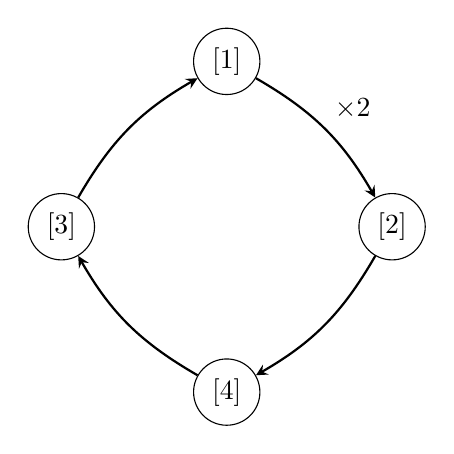
\begin{tikzpicture}[>=stealth,scale=1.05]
\node[circle,draw] (1) at (0,2) {\([1]\)};
\node[circle,draw] (2) at (2,0) {\([2]\)};
\node[circle,draw] (4) at (0,-2) {\([4]\)};
\node[circle,draw] (3) at (-2,0) {\([3]\)};

\draw[->,thick] (1) to[bend left=15] node[above right]{\(\times2\)} (2);
\draw[->,thick] (2) to[bend left=15] (4);
\draw[->,thick] (4) to[bend left=15] (3);
\draw[->,thick] (3) to[bend left=15] (1);
\end{tikzpicture}
\end{center}

Repeated multiplication by \([2]_5\) gives

\[ [1]\to[2]\to[4]\to[3]\to[1]. \]

Thus \([2]_5\) generates the multiplicative group

\[ \F_5^\times. \]

%%%%%%%%%%%%%%%%%%%%%%%%%%%%%%%%%%%%%%%%%%%%%%%%%%%%%%%%%%%%
\subsection{Characteristic of a Field}
\label{subsec:field-characteristic}
%%%%%%%%%%%%%%%%%%%%%%%%%%%%%%%%%%%%%%%%%%%%%%%%%%%%%%%%%%%%

Characteristic was introduced for rings in
\cref{subsec:ring-characteristic}.

For a field \(F\),

\[ \operatorname{char}(F) \]

is the smallest positive integer \(n\) satisfying

\[ n\cdot1_F=0, \]

if such an integer exists.

Otherwise,

\[ \operatorname{char}(F)=0. \]

%%%%%%%%%%%%%%%%%%%%%%%%%%%%%%%%%%%%%%%%%%%%%%%%%%%%%%%%%%%%
\subsection{Possible Characteristics of Fields}
\label{subsec:field-characteristic-prime}
%%%%%%%%%%%%%%%%%%%%%%%%%%%%%%%%%%%%%%%%%%%%%%%%%%%%%%%%%%%%

\begin{theorem}
The characteristic of a field is either \(0\) or a prime number.
\end{theorem}

This follows because every field is an integral domain, and the
characteristic of an integral domain is either \(0\) or prime.

Thus no field can have characteristic

\[ 4,\quad6,\quad8,\quad9,\quad10,\ldots \]

or any other positive composite integer.

%%%%%%%%%%%%%%%%%%%%%%%%%%%%%%%%%%%%%%%%%%%%%%%%%%%%%%%%%%%%
\subsection{Examples of Field Characteristics}
\label{subsec:field-characteristic-examples}
%%%%%%%%%%%%%%%%%%%%%%%%%%%%%%%%%%%%%%%%%%%%%%%%%%%%%%%%%%%%

The familiar infinite fields satisfy

\[ \operatorname{char}(\Q)=0,\qquad \operatorname{char}(\R)=0,\qquad \operatorname{char}(\C)=0. \]

For a prime \(p\),

\[ \operatorname{char}(\F_p)=p. \]

For example,

\[ \operatorname{char}(\F_7)=7. \]

%%%%%%%%%%%%%%%%%%%%%%%%%%%%%%%%%%%%%%%%%%%%%%%%%%%%%%%%%%%%
\subsection{Prime Subfields}
\label{subsec:prime-subfields}
%%%%%%%%%%%%%%%%%%%%%%%%%%%%%%%%%%%%%%%%%%%%%%%%%%%%%%%%%%%%

Every field contains a smallest subfield.

\begin{definitionbox}{Prime Subfield}
The \emph{prime subfield} of a field \(F\) is the smallest subfield contained
in \(F\).
\end{definitionbox}

Its form is completely determined by the characteristic.

If

\[ \operatorname{char}(F)=0, \]

then the prime subfield is isomorphic to

\[ \Q. \]

If

\[ \operatorname{char}(F)=p, \]

then the prime subfield is isomorphic to

\[ \F_p. \]

%%%%%%%%%%%%%%%%%%%%%%%%%%%%%%%%%%%%%%%%%%%%%%%%%%%%%%%%%%%%
\subsection{Visualizing Prime Subfields}
\label{subsec:visual-prime-subfields}
%%%%%%%%%%%%%%%%%%%%%%%%%%%%%%%%%%%%%%%%%%%%%%%%%%%%%%%%%%%%

\begin{center}
\begin{tikzpicture}[
    node distance=12mm,
    box/.style={draw,rounded corners,align=center,inner sep=5pt,font=\small},
    >=stealth
]
\node[box] (F) {Field \(F\)};
\node[box,below left=of F] (zero) {\(\operatorname{char}(F)=0\)};
\node[box,below right=of F] (p) {\(\operatorname{char}(F)=p\)};
\node[box,below=of zero] (Q) {contains a copy of \(\Q\)};
\node[box,below=of p] (Fp) {contains a copy of \(\F_p\)};

\draw[->] (F)--(zero);
\draw[->] (F)--(p);
\draw[->] (zero)--(Q);
\draw[->] (p)--(Fp);
\end{tikzpicture}
\end{center}

%%%%%%%%%%%%%%%%%%%%%%%%%%%%%%%%%%%%%%%%%%%%%%%%%%%%%%%%%%%%
\subsection{Subfields}
\label{subsec:subfields}
%%%%%%%%%%%%%%%%%%%%%%%%%%%%%%%%%%%%%%%%%%%%%%%%%%%%%%%%%%%%

\begin{definitionbox}{Subfield}
A subset \(K\subseteq F\) is a \emph{subfield} of \(F\) if \(K\) itself forms
a field under the operations inherited from \(F\).
\end{definitionbox}

For example,

\[ \Q\subseteq\R\subseteq\C. \]

Thus \(\Q\) is a subfield of \(\R\), and \(\R\) is a subfield of \(\C\).

%%%%%%%%%%%%%%%%%%%%%%%%%%%%%%%%%%%%%%%%%%%%%%%%%%%%%%%%%%%%
\subsection{Subfield Test}
\label{subsec:subfield-test}
%%%%%%%%%%%%%%%%%%%%%%%%%%%%%%%%%%%%%%%%%%%%%%%%%%%%%%%%%%%%

\begin{theorem}[Subfield Test]
Let \(K\) be a subset of a field \(F\) containing at least two elements.

Then \(K\) is a subfield if, whenever \(a,b\in K\),

\[ a-b\in K \]

and, whenever \(b\neq0\),

\[ ab^{-1}\in K. \]
\end{theorem}

These conditions guarantee closure under subtraction and division by nonzero
elements.

%%%%%%%%%%%%%%%%%%%%%%%%%%%%%%%%%%%%%%%%%%%%%%%%%%%%%%%%%%%%
\subsection{Field Extensions}
\label{subsec:field-extensions}
%%%%%%%%%%%%%%%%%%%%%%%%%%%%%%%%%%%%%%%%%%%%%%%%%%%%%%%%%%%%

A central idea of field theory is to enlarge a field by adding new elements.

\begin{definitionbox}{Field Extension}
If \(K\) is a subfield of \(L\), then \(L\) is called a \emph{field
extension} of \(K\).

The extension is written
\[ L/K. \]
\end{definitionbox}

The notation

\[ L/K \]

is read ``L over K.''

It does not denote ordinary division.

It means that \(K\) is being regarded as a subfield of \(L\).

%%%%%%%%%%%%%%%%%%%%%%%%%%%%%%%%%%%%%%%%%%%%%%%%%%%%%%%%%%%%
\subsection{Visualizing a Field Extension}
\label{subsec:visual-field-extension}
%%%%%%%%%%%%%%%%%%%%%%%%%%%%%%%%%%%%%%%%%%%%%%%%%%%%%%%%%%%%

\begin{center}
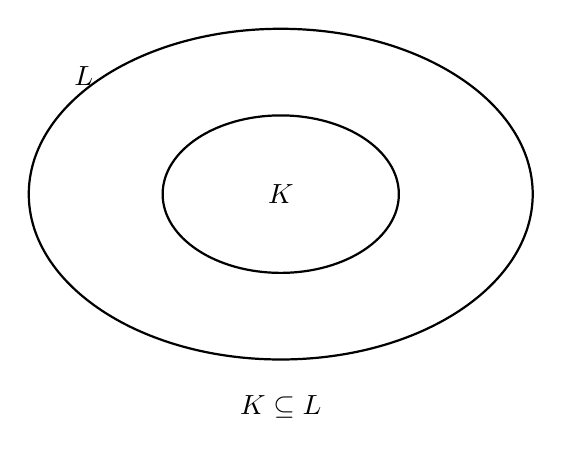
\begin{tikzpicture}
\draw[thick] (0,0) ellipse (3.2 and 2.1);
\draw[thick] (0,0) ellipse (1.5 and 1);

\node at (-2.5,1.5) {\(L\)};
\node at (0,0) {\(K\)};
\node at (0,-2.7) {\(K\subseteq L\)};
\end{tikzpicture}
\end{center}

The larger field contains all elements and operations of the smaller field,
together with additional elements.

%%%%%%%%%%%%%%%%%%%%%%%%%%%%%%%%%%%%%%%%%%%%%%%%%%%%%%%%%%%%
\subsection{Examples of Field Extensions}
\label{subsec:field-extension-examples}
%%%%%%%%%%%%%%%%%%%%%%%%%%%%%%%%%%%%%%%%%%%%%%%%%%%%%%%%%%%%

The inclusions

\[ \Q\subseteq\R\subseteq\C \]

produce extensions

\[ \R/\Q,\qquad \C/\R,\qquad \C/\Q. \]

Another important example is

\[ \Q(\sqrt2)/\Q. \]

The field \(\Q(\sqrt2)\) is obtained by adjoining \(\sqrt2\) to the rational
numbers.

%%%%%%%%%%%%%%%%%%%%%%%%%%%%%%%%%%%%%%%%%%%%%%%%%%%%%%%%%%%%
\subsection{Adjoining an Element}
\label{subsec:adjoining-field-element}
%%%%%%%%%%%%%%%%%%%%%%%%%%%%%%%%%%%%%%%%%%%%%%%%%%%%%%%%%%%%

Suppose \(L/K\) is a field extension and \(\alpha\in L\).

\begin{definitionbox}{Simple Field Extension}
The field
\[ K(\alpha) \]
is the smallest subfield of \(L\) containing both \(K\) and \(\alpha\).

An extension of the form
\[ K(\alpha)/K \]
is called a \emph{simple extension}.
\end{definitionbox}

The symbol

\[ \alpha \]

is lowercase Greek \emph{alpha}, pronounced ``AL-fuh.''

The notation

\[ K(\alpha) \]

is read ``K adjoin alpha.''

%%%%%%%%%%%%%%%%%%%%%%%%%%%%%%%%%%%%%%%%%%%%%%%%%%%%%%%%%%%%
\subsection{Example: \(\Q(\sqrt2)\)}
\label{subsec:q-sqrt2}
%%%%%%%%%%%%%%%%%%%%%%%%%%%%%%%%%%%%%%%%%%%%%%%%%%%%%%%%%%%%

Because

\[ (\sqrt2)^2=2, \]

higher powers of \(\sqrt2\) reduce to combinations of \(1\) and \(\sqrt2\).

Thus

\[ \Q(\sqrt2)=\{a+b\sqrt2:a,b\in\Q\}. \]

For example,

\[ 3+\frac52\sqrt2\in\Q(\sqrt2). \]

%%%%%%%%%%%%%%%%%%%%%%%%%%%%%%%%%%%%%%%%%%%%%%%%%%%%%%%%%%%%
\subsection{Why \(\Q(\sqrt2)\) Is Closed Under Inverses}
\label{subsec:q-sqrt2-inverses}
%%%%%%%%%%%%%%%%%%%%%%%%%%%%%%%%%%%%%%%%%%%%%%%%%%%%%%%%%%%%

Take

\[ a+b\sqrt2\neq0. \]

Multiply numerator and denominator by its conjugate:

\[ \frac{1}{a+b\sqrt2}=\frac{a-b\sqrt2}{a^2-2b^2}. \]

Since \(a,b\in\Q\),

\[ a^2-2b^2\in\Q. \]

For a nonzero element, this denominator is nonzero.

Therefore,

\[ \frac{1}{a+b\sqrt2}\in\Q(\sqrt2). \]

So the set is closed under multiplicative inverses of nonzero elements.

%%%%%%%%%%%%%%%%%%%%%%%%%%%%%%%%%%%%%%%%%%%%%%%%%%%%%%%%%%%%
\subsection{Field Extensions as Vector Spaces}
\label{subsec:extensions-vector-spaces}
%%%%%%%%%%%%%%%%%%%%%%%%%%%%%%%%%%%%%%%%%%%%%%%%%%%%%%%%%%%%

One of the most important connections between field theory and linear algebra
is that a field extension naturally forms a vector space.

If

\[ K\subseteq L, \]

then \(L\) can be viewed as a vector space over \(K\).

Vector addition is the ordinary addition in \(L\).

Scalar multiplication is multiplication by elements of \(K\).

%%%%%%%%%%%%%%%%%%%%%%%%%%%%%%%%%%%%%%%%%%%%%%%%%%%%%%%%%%%%
\subsection{Degree of a Field Extension}
\label{subsec:degree-field-extension}
%%%%%%%%%%%%%%%%%%%%%%%%%%%%%%%%%%%%%%%%%%%%%%%%%%%%%%%%%%%%

\begin{definitionbox}{Degree of a Field Extension}
The \emph{degree} of an extension \(L/K\) is the vector-space dimension of
\(L\) over \(K\):
\[ [L:K]=\dim_K L. \]
\end{definitionbox}

The notation

\[ [L:K] \]

is read ``the degree of L over K.''

Notice that square brackets are used here for extension degree, while the same
notation in group theory may represent subgroup index. Context determines the
meaning.

%%%%%%%%%%%%%%%%%%%%%%%%%%%%%%%%%%%%%%%%%%%%%%%%%%%%%%%%%%%%
\subsection{Degree of \(\Q(\sqrt2)/\Q\)}
\label{subsec:degree-q-sqrt2}
%%%%%%%%%%%%%%%%%%%%%%%%%%%%%%%%%%%%%%%%%%%%%%%%%%%%%%%%%%%%

Every element of \(\Q(\sqrt2)\) has the form

\[ a+b\sqrt2. \]

Thus

\[ \{1,\sqrt2\} \]

spans \(\Q(\sqrt2)\) over \(\Q\).

The elements \(1\) and \(\sqrt2\) are linearly independent over \(\Q\).

Therefore,

\[ \{1,\sqrt2\} \]

is a basis and

\[ [\Q(\sqrt2):\Q]=2. \]

%%%%%%%%%%%%%%%%%%%%%%%%%%%%%%%%%%%%%%%%%%%%%%%%%%%%%%%%%%%%
\subsection{Visualizing Extension Degree}
\label{subsec:visual-extension-degree}
%%%%%%%%%%%%%%%%%%%%%%%%%%%%%%%%%%%%%%%%%%%%%%%%%%%%%%%%%%%%

\begin{center}
\begin{tikzpicture}[
    node distance=12mm,
    box/.style={draw,rounded corners,align=center,inner sep=6pt},
    >=stealth
]
\node[box] (Q) {\(\Q\)};
\node[box,above=of Q] (L) {\(\Q(\sqrt2)\)};

\draw[->,thick] (Q)--node[right]{degree \(2\)}(L);

\node[right=20mm of L] {\(\{1,\sqrt2\}\)};
\node[right=20mm of Q] {basis over \(\Q\)};
\end{tikzpicture}
\end{center}

The degree counts how many basis directions are needed when the larger field
is viewed as a vector space over the smaller field.

%%%%%%%%%%%%%%%%%%%%%%%%%%%%%%%%%%%%%%%%%%%%%%%%%%%%%%%%%%%%
\subsection{Finite and Infinite Extensions}
\label{subsec:finite-infinite-extensions}
%%%%%%%%%%%%%%%%%%%%%%%%%%%%%%%%%%%%%%%%%%%%%%%%%%%%%%%%%%%%

\begin{definitionbox}{Finite Extension}
An extension \(L/K\) is \emph{finite} if
\[ [L:K]<\infty. \]

Otherwise it is called an \emph{infinite extension}.
\end{definitionbox}

For example,

\[ [\C:\R]=2 \]

because

\[ \C=\{a+bi:a,b\in\R\}. \]

A basis is

\[ \{1,i\}. \]

%%%%%%%%%%%%%%%%%%%%%%%%%%%%%%%%%%%%%%%%%%%%%%%%%%%%%%%%%%%%
\subsection{The Tower Law}
\label{subsec:tower-law}
%%%%%%%%%%%%%%%%%%%%%%%%%%%%%%%%%%%%%%%%%%%%%%%%%%%%%%%%%%%%

Field extensions can be stacked.

Suppose

\[ K\subseteq L\subseteq M. \]

Then \(M\) is an extension of \(L\), and \(L\) is an extension of \(K\).

\begin{theorem}[Tower Law]
If the relevant degrees are finite, then
\[ [M:K]=[M:L][L:K]. \]
\end{theorem}

%%%%%%%%%%%%%%%%%%%%%%%%%%%%%%%%%%%%%%%%%%%%%%%%%%%%%%%%%%%%
\subsection{Visualizing the Tower Law}
\label{subsec:visual-tower-law}
%%%%%%%%%%%%%%%%%%%%%%%%%%%%%%%%%%%%%%%%%%%%%%%%%%%%%%%%%%%%

\begin{center}
\begin{tikzpicture}[
    node distance=13mm,
    box/.style={draw,rounded corners,minimum width=18mm,minimum height=8mm},
    >=stealth
]
\node[box] (K) {\(K\)};
\node[box,above=of K] (L) {\(L\)};
\node[box,above=of L] (M) {\(M\)};

\draw[->,thick] (K)--node[right]{\([L:K]\)}(L);
\draw[->,thick] (L)--node[right]{\([M:L]\)}(M);

\draw[->,thick,bend left=55] (K) to node[left]{\([M:K]\)} (M);
\end{tikzpicture}
\end{center}

The degrees multiply:

\[ [M:K]=[M:L][L:K]. \]

%%%%%%%%%%%%%%%%%%%%%%%%%%%%%%%%%%%%%%%%%%%%%%%%%%%%%%%%%%%%
\subsection{Worked Example: Using the Tower Law}
\label{subsec:worked-tower-law}
%%%%%%%%%%%%%%%%%%%%%%%%%%%%%%%%%%%%%%%%%%%%%%%%%%%%%%%%%%%%

\begin{workedexamplebox}{Computing an Extension Degree}

Suppose

\[ K\subseteq L\subseteq M \]

with

\[ [L:K]=3,\qquad[M:L]=4. \]

Find \([M:K]\).

\begin{tabularx}{\textwidth}{@{}>{\raggedright\arraybackslash}p{0.42\textwidth}X@{}}
Use the Tower Law. & \([M:K]=[M:L][L:K]\)\\
Substitute the degrees. & \([M:K]=4\cdot3\)\\
Multiply. & \([M:K]=12\)
\end{tabularx}

\begin{answerbox}
\[ [M:K]=12. \]
\end{answerbox}
\end{workedexamplebox}

%%%%%%%%%%%%%%%%%%%%%%%%%%%%%%%%%%%%%%%%%%%%%%%%%%%%%%%%%%%%
\subsection{Algebraic Elements}
\label{subsec:algebraic-elements}
%%%%%%%%%%%%%%%%%%%%%%%%%%%%%%%%%%%%%%%%%%%%%%%%%%%%%%%%%%%%

Suppose \(L/K\) is a field extension and \(\alpha\in L\).

\begin{definitionbox}{Algebraic Element}
The element \(\alpha\) is \emph{algebraic over \(K\)} if there exists a
nonzero polynomial
\[ f(x)\in K[x] \]
such that
\[ f(\alpha)=0. \]
\end{definitionbox}

For example,

\[ \sqrt2 \]

is algebraic over \(\Q\) because it satisfies

\[ x^2-2=0. \]

%%%%%%%%%%%%%%%%%%%%%%%%%%%%%%%%%%%%%%%%%%%%%%%%%%%%%%%%%%%%
\subsection{Transcendental Elements}
\label{subsec:transcendental-elements}
%%%%%%%%%%%%%%%%%%%%%%%%%%%%%%%%%%%%%%%%%%%%%%%%%%%%%%%%%%%%

\begin{definitionbox}{Transcendental Element}
An element \(\alpha\in L\) is \emph{transcendental over \(K\)} if it is not
algebraic over \(K\).
\end{definitionbox}

Thus no nonzero polynomial in \(K[x]\) has \(\alpha\) as a root.

The numbers

\[ \pi\qquad\text{and}\qquad e \]

are transcendental over \(\Q\).

Here \(\pi\) is the Greek letter \emph{pi}, pronounced ``pie,'' and \(e\)
denotes Euler's number.

%%%%%%%%%%%%%%%%%%%%%%%%%%%%%%%%%%%%%%%%%%%%%%%%%%%%%%%%%%%%
\subsection{Algebraic Versus Transcendental}
\label{subsec:algebraic-transcendental-visual}
%%%%%%%%%%%%%%%%%%%%%%%%%%%%%%%%%%%%%%%%%%%%%%%%%%%%%%%%%%%%

\begin{center}
\begin{tikzpicture}[
    node distance=12mm and 20mm,
    box/.style={draw,rounded corners,align=center,inner sep=5pt},
    >=stealth
]
\node[box] (alpha) {Element \(\alpha\)\\over \(K\)};
\node[box,below left=of alpha] (alg) {Algebraic};
\node[box,below right=of alpha] (trans) {Transcendental};

\node[below=5mm of alg,align=center] {\(\exists\,0\neq f\in K[x]\)\\with \(f(\alpha)=0\)};
\node[below=5mm of trans,align=center] {no such polynomial\\exists};

\draw[->] (alpha)--(alg);
\draw[->] (alpha)--(trans);
\end{tikzpicture}
\end{center}

The symbol

\[ \exists \]

is the existential quantifier and is read ``there exists.''

%%%%%%%%%%%%%%%%%%%%%%%%%%%%%%%%%%%%%%%%%%%%%%%%%%%%%%%%%%%%
\subsection{Minimal Polynomials}
\label{subsec:minimal-polynomials}
%%%%%%%%%%%%%%%%%%%%%%%%%%%%%%%%%%%%%%%%%%%%%%%%%%%%%%%%%%%%

If \(\alpha\) is algebraic over \(K\), many polynomials may vanish at
\(\alpha\).

Among them, one is structurally fundamental.

\begin{definitionbox}{Minimal Polynomial}
Let \(\alpha\) be algebraic over \(K\). The \emph{minimal polynomial} of
\(\alpha\) over \(K\) is the unique monic polynomial of smallest positive
degree
\[ m_{\alpha,K}(x)\in K[x] \]
such that
\[ m_{\alpha,K}(\alpha)=0. \]
\end{definitionbox}

The notation

\[ m_{\alpha,K}(x) \]

is read ``the minimal polynomial of alpha over K.''

%%%%%%%%%%%%%%%%%%%%%%%%%%%%%%%%%%%%%%%%%%%%%%%%%%%%%%%%%%%%
\subsection{Example of a Minimal Polynomial}
\label{subsec:minimal-polynomial-sqrt2}
%%%%%%%%%%%%%%%%%%%%%%%%%%%%%%%%%%%%%%%%%%%%%%%%%%%%%%%%%%%%

For

\[ \alpha=\sqrt2 \]

over \(\Q\),

\[ x^2-2 \]

has \(\sqrt2\) as a root.

It is irreducible over \(\Q\).

Therefore,

\[ m_{\sqrt2,\Q}(x)=x^2-2. \]

Its degree is \(2\).

Correspondingly,

\[ [\Q(\sqrt2):\Q]=2. \]

%%%%%%%%%%%%%%%%%%%%%%%%%%%%%%%%%%%%%%%%%%%%%%%%%%%%%%%%%%%%
\subsection{Minimal Polynomial and Extension Degree}
\label{subsec:minimal-polynomial-extension-degree}
%%%%%%%%%%%%%%%%%%%%%%%%%%%%%%%%%%%%%%%%%%%%%%%%%%%%%%%%%%%%

\begin{theorem}
If \(\alpha\) is algebraic over \(K\), then
\[ [K(\alpha):K]=\deg m_{\alpha,K}. \]
\end{theorem}

Thus the degree of the minimal polynomial determines the dimension of the
simple extension.

If

\[ \deg m_{\alpha,K}=n, \]

then a standard basis is

\[ \{1,\alpha,\alpha^2,\ldots,\alpha^{n-1}\}. \]

%%%%%%%%%%%%%%%%%%%%%%%%%%%%%%%%%%%%%%%%%%%%%%%%%%%%%%%%%%%%
\subsection{Visualizing the Minimal Polynomial Connection}
\label{subsec:visual-minimal-polynomial}
%%%%%%%%%%%%%%%%%%%%%%%%%%%%%%%%%%%%%%%%%%%%%%%%%%%%%%%%%%%%

\begin{center}
\begin{tikzpicture}[
    node distance=12mm,
    box/.style={draw,rounded corners,align=center,inner sep=5pt},
    >=stealth
]
\node[box] (poly) {Minimal polynomial\\\(m_{\alpha,K}(x)\)};
\node[box,right=of poly] (degree) {Degree \(n\)};
\node[box,right=of degree] (basis) {\(1,\alpha,\ldots,\alpha^{n-1}\)};
\node[box,right=of basis] (ext) {\([K(\alpha):K]=n\)};

\draw[->,thick] (poly)--(degree);
\draw[->,thick] (degree)--(basis);
\draw[->,thick] (basis)--(ext);
\end{tikzpicture}
\end{center}

%%%%%%%%%%%%%%%%%%%%%%%%%%%%%%%%%%%%%%%%%%%%%%%%%%%%%%%%%%%%
\subsection{Worked Example: \(\Q(\sqrt3)\)}
\label{subsec:worked-q-sqrt3}
%%%%%%%%%%%%%%%%%%%%%%%%%%%%%%%%%%%%%%%%%%%%%%%%%%%%%%%%%%%%

\begin{workedexamplebox}{A Quadratic Field Extension}

Determine the minimal polynomial and extension degree of \(\sqrt3\) over
\(\Q\).

\begin{tabularx}{\textwidth}{@{}>{\raggedright\arraybackslash}p{0.42\textwidth}X@{}}
Find a polynomial satisfied by \(\sqrt3\). & \((\sqrt3)^2-3=0\)\\
Write the polynomial. & \(f(x)=x^2-3\)\\
Observe that \(x^2-3\) is irreducible over \(\Q\). & \(m_{\sqrt3,\Q}(x)=x^2-3\)\\
Use its degree. & \([\Q(\sqrt3):\Q]=2\)
\end{tabularx}

\begin{answerbox}
\[ m_{\sqrt3,\Q}(x)=x^2-3,\qquad[\Q(\sqrt3):\Q]=2. \]
\end{answerbox}
\end{workedexamplebox}

%%%%%%%%%%%%%%%%%%%%%%%%%%%%%%%%%%%%%%%%%%%%%%%%%%%%%%%%%%%%
\subsection{Finite Extensions Are Algebraic}
\label{subsec:finite-extensions-algebraic}
%%%%%%%%%%%%%%%%%%%%%%%%%%%%%%%%%%%%%%%%%%%%%%%%%%%%%%%%%%%%

\begin{theorem}
Every finite field extension is algebraic.
\end{theorem}

\begin{proof}
Suppose

\[ [L:K]=n<\infty. \]

Take \(\alpha\in L\).

The \(n+1\) elements

\[ 1,\alpha,\alpha^2,\ldots,\alpha^n \]

belong to the \(n\)-dimensional vector space \(L\) over \(K\).

Therefore they are linearly dependent.

Hence there exist coefficients

\[ a_0,a_1,\ldots,a_n\in K, \]

not all zero, such that

\[ a_0+a_1\alpha+\cdots+a_n\alpha^n=0. \]

Thus \(\alpha\) satisfies a nonzero polynomial over \(K\).

Therefore \(\alpha\) is algebraic over \(K\).
\end{proof}

%%%%%%%%%%%%%%%%%%%%%%%%%%%%%%%%%%%%%%%%%%%%%%%%%%%%%%%%%%%%
\subsection{The Converse Is Not Always True}
\label{subsec:algebraic-not-finite}
%%%%%%%%%%%%%%%%%%%%%%%%%%%%%%%%%%%%%%%%%%%%%%%%%%%%%%%%%%%%

An extension may be algebraic without being finite.

Thus

\[ \text{finite extension}\Longrightarrow\text{algebraic extension}, \]

but the converse is not generally true.

This distinction becomes important when infinitely many algebraic elements
are adjoined.

%%%%%%%%%%%%%%%%%%%%%%%%%%%%%%%%%%%%%%%%%%%%%%%%%%%%%%%%%%%%
\subsection{Algebraic Extensions}
\label{subsec:algebraic-extensions}
%%%%%%%%%%%%%%%%%%%%%%%%%%%%%%%%%%%%%%%%%%%%%%%%%%%%%%%%%%%%

\begin{definitionbox}{Algebraic Extension}
An extension \(L/K\) is \emph{algebraic} if every element of \(L\) is
algebraic over \(K\).
\end{definitionbox}

If at least one element of \(L\) is transcendental over \(K\), the extension
is not algebraic.

%%%%%%%%%%%%%%%%%%%%%%%%%%%%%%%%%%%%%%%%%%%%%%%%%%%%%%%%%%%%
\subsection{Transcendental Extensions}
\label{subsec:transcendental-extensions}
%%%%%%%%%%%%%%%%%%%%%%%%%%%%%%%%%%%%%%%%%%%%%%%%%%%%%%%%%%%%

An extension containing elements transcendental over the base field is called
a \emph{transcendental extension}.

For example,

\[ \R/\Q \]

is transcendental because \(\R\) contains transcendental numbers such as
\(\pi\).

%%%%%%%%%%%%%%%%%%%%%%%%%%%%%%%%%%%%%%%%%%%%%%%%%%%%%%%%%%%%
\subsection{Polynomial Quotients as Fields}
\label{subsec:polynomial-quotient-fields}
%%%%%%%%%%%%%%%%%%%%%%%%%%%%%%%%%%%%%%%%%%%%%%%%%%%%%%%%%%%%

Ring theory showed that if \(F\) is a field and \(p(x)\in F[x]\) is
irreducible, then

\[ (p(x)) \]

is a maximal ideal of \(F[x]\).

Therefore,

\[ F[x]/(p(x)) \]

is a field.

This provides one of the most important methods for constructing new fields.

%%%%%%%%%%%%%%%%%%%%%%%%%%%%%%%%%%%%%%%%%%%%%%%%%%%%%%%%%%%%
\subsection{Constructing \(\C\) from \(\R\)}
\label{subsec:constructing-complex-field}
%%%%%%%%%%%%%%%%%%%%%%%%%%%%%%%%%%%%%%%%%%%%%%%%%%%%%%%%%%%%

The polynomial

\[ x^2+1 \]

has no real roots and is irreducible over \(\R\).

Therefore,

\[ \R[x]/(x^2+1) \]

is a field.

Inside this quotient,

\[ [x]^2=[-1]. \]

Thus the residue class \([x]\) behaves like the imaginary unit \(i\).

Consequently,

\[ \R[x]/(x^2+1)\cong\C. \]

%%%%%%%%%%%%%%%%%%%%%%%%%%%%%%%%%%%%%%%%%%%%%%%%%%%%%%%%%%%%
\subsection{Visualizing Field Construction by Quotient}
\label{subsec:visual-field-quotient-construction}
%%%%%%%%%%%%%%%%%%%%%%%%%%%%%%%%%%%%%%%%%%%%%%%%%%%%%%%%%%%%

\begin{center}
\begin{tikzpicture}[
    node distance=13mm,
    box/.style={draw,rounded corners,align=center,inner sep=5pt},
    >=stealth
]
\node[box] (R) {\(\R\)};
\node[box,right=of R] (poly) {\(\R[x]\)};
\node[box,right=of poly] (quot) {\(\R[x]/(x^2+1)\)};
\node[box,right=of quot] (C) {\(\C\)};

\draw[->,thick] (R)--node[above]{polynomials}(poly);
\draw[->,thick] (poly)--node[above]{impose \(x^2=-1\)}(quot);
\draw[->,thick] (quot)--node[above]{\(\cong\)}(C);
\end{tikzpicture}
\end{center}

This construction turns a formal root of \(x^2+1\) into an actual field
element.

%%%%%%%%%%%%%%%%%%%%%%%%%%%%%%%%%%%%%%%%%%%%%%%%%%%%%%%%%%%%
\subsection{Adjoining a Root of an Irreducible Polynomial}
\label{subsec:adjoining-irreducible-root}
%%%%%%%%%%%%%%%%%%%%%%%%%%%%%%%%%%%%%%%%%%%%%%%%%%%%%%%%%%%%

Let

\[ p(x)\in F[x] \]

be irreducible.

Construct

\[ E=F[x]/(p(x)). \]

Let

\[ \alpha=[x]. \]

Then

\[ p(\alpha)=0. \]

Thus \(E\) contains a root of \(p(x)\), even if \(F\) originally did not.

\begin{conceptbox}
Field extensions allow algebra to create new number systems in which
previously unsolvable polynomial equations acquire solutions.
\end{conceptbox}

%%%%%%%%%%%%%%%%%%%%%%%%%%%%%%%%%%%%%%%%%%%%%%%%%%%%%%%%%%%%
\subsection{Example: Adjoining \(\sqrt2\)}
\label{subsec:quotient-q-sqrt2}
%%%%%%%%%%%%%%%%%%%%%%%%%%%%%%%%%%%%%%%%%%%%%%%%%%%%%%%%%%%%

The polynomial

\[ x^2-2 \]

is irreducible over \(\Q\).

Therefore,

\[ \Q[x]/(x^2-2) \]

is a field.

If

\[ \alpha=[x], \]

then

\[ \alpha^2=2. \]

Hence \(\alpha\) behaves like \(\sqrt2\), and

\[ \Q[x]/(x^2-2)\cong\Q(\sqrt2). \]

%%%%%%%%%%%%%%%%%%%%%%%%%%%%%%%%%%%%%%%%%%%%%%%%%%%%%%%%%%%%
\subsection{Splitting Fields}
\label{subsec:splitting-fields}
%%%%%%%%%%%%%%%%%%%%%%%%%%%%%%%%%%%%%%%%%%%%%%%%%%%%%%%%%%%%

A polynomial may require several new elements before all of its roots appear.

\begin{definitionbox}{Splitting Field}
Let \(f(x)\in K[x]\). A \emph{splitting field} of \(f\) over \(K\) is a
smallest field extension \(L/K\) in which \(f(x)\) factors completely into
linear factors.
\end{definitionbox}

Thus in \(L[x]\),

\[ f(x)=a(x-\alpha_1)(x-\alpha_2)\cdots(x-\alpha_n). \]

%%%%%%%%%%%%%%%%%%%%%%%%%%%%%%%%%%%%%%%%%%%%%%%%%%%%%%%%%%%%
\subsection{Example: Splitting \(x^2-2\)}
\label{subsec:splitting-x2-minus2}
%%%%%%%%%%%%%%%%%%%%%%%%%%%%%%%%%%%%%%%%%%%%%%%%%%%%%%%%%%%%

Over \(\Q\),

\[ x^2-2 \]

does not split into linear factors.

After adjoining \(\sqrt2\),

\[ x^2-2=(x-\sqrt2)(x+\sqrt2). \]

Therefore,

\[ \Q(\sqrt2) \]

is the splitting field of \(x^2-2\) over \(\Q\).

%%%%%%%%%%%%%%%%%%%%%%%%%%%%%%%%%%%%%%%%%%%%%%%%%%%%%%%%%%%%
\subsection{Example: Splitting \(x^2+1\)}
\label{subsec:splitting-x2-plus1}
%%%%%%%%%%%%%%%%%%%%%%%%%%%%%%%%%%%%%%%%%%%%%%%%%%%%%%%%%%%%

Over \(\R\),

\[ x^2+1 \]

has no roots.

In \(\C\),

\[ x^2+1=(x-i)(x+i). \]

Therefore,

\[ \C \]

is the splitting field of \(x^2+1\) over \(\R\).

%%%%%%%%%%%%%%%%%%%%%%%%%%%%%%%%%%%%%%%%%%%%%%%%%%%%%%%%%%%%
\subsection{Visualizing a Splitting Field}
\label{subsec:visual-splitting-field}
%%%%%%%%%%%%%%%%%%%%%%%%%%%%%%%%%%%%%%%%%%%%%%%%%%%%%%%%%%%%

\begin{center}
\begin{tikzpicture}[
    node distance=14mm,
    box/.style={draw,rounded corners,align=center,inner sep=6pt},
    >=stealth
]
\node[box] (K) {Base field \(K\)};
\node[box,above=of K] (L) {Splitting field \(L\)};
\node[left=18mm of K] (f) {\(f(x)\)};
\node[right=18mm of L] (split) {\(a\prod_{j=1}^{n}(x-\alpha_j)\)};

\draw[->,thick] (K)--node[right]{adjoin roots}(L);
\draw[->,thick] (f)--(K);
\draw[->,thick] (L)--(split);
\end{tikzpicture}
\end{center}

The symbol

\[ \prod \]

is the capital Greek product symbol, called \emph{product notation}, and is
read ``the product.''

Thus

\[ \prod_{j=1}^{n}(x-\alpha_j) \]

is read ``the product from \(j=1\) to \(n\) of \(x-\alpha_j\).''

%%%%%%%%%%%%%%%%%%%%%%%%%%%%%%%%%%%%%%%%%%%%%%%%%%%%%%%%%%%%
\subsection{Algebraically Closed Fields}
\label{subsec:algebraically-closed-fields}
%%%%%%%%%%%%%%%%%%%%%%%%%%%%%%%%%%%%%%%%%%%%%%%%%%%%%%%%%%%%

\begin{definitionbox}{Algebraically Closed Field}
A field \(F\) is \emph{algebraically closed} if every nonconstant polynomial
in \(F[x]\) has a root in \(F\).
\end{definitionbox}

Equivalently, every nonconstant polynomial in \(F[x]\) factors completely
into linear factors over \(F\).

The complex numbers provide the most familiar example.

%%%%%%%%%%%%%%%%%%%%%%%%%%%%%%%%%%%%%%%%%%%%%%%%%%%%%%%%%%%%
\subsection{The Fundamental Theorem of Algebra}
\label{subsec:fundamental-theorem-algebra-field}
%%%%%%%%%%%%%%%%%%%%%%%%%%%%%%%%%%%%%%%%%%%%%%%%%%%%%%%%%%%%

\begin{theorem}[Fundamental Theorem of Algebra]
Every nonconstant polynomial with complex coefficients has at least one
complex root.
\end{theorem}

Consequently,

\[ \C \]

is algebraically closed.

A polynomial of degree \(n\) over \(\C\) factors as

\[ f(x)=a(x-\alpha_1)\cdots(x-\alpha_n), \]

where roots are counted with multiplicity.

%%%%%%%%%%%%%%%%%%%%%%%%%%%%%%%%%%%%%%%%%%%%%%%%%%%%%%%%%%%%
\subsection{Algebraic Closure}
\label{subsec:algebraic-closure}
%%%%%%%%%%%%%%%%%%%%%%%%%%%%%%%%%%%%%%%%%%%%%%%%%%%%%%%%%%%%

\begin{definitionbox}{Algebraic Closure}
An \emph{algebraic closure} of a field \(F\) is an algebraic extension
\(\overline{F}/F\) such that \(\overline{F}\) is algebraically closed.
\end{definitionbox}

The notation

\[ \overline{F} \]

is read ``F bar.''

For example,

\[ \overline{\Q} \]

denotes the field of algebraic numbers over \(\Q\) inside a chosen algebraic
closure.

%%%%%%%%%%%%%%%%%%%%%%%%%%%%%%%%%%%%%%%%%%%%%%%%%%%%%%%%%%%%
\subsection{Field Extension Diagram}
\label{subsec:field-extension-diagram}
%%%%%%%%%%%%%%%%%%%%%%%%%%%%%%%%%%%%%%%%%%%%%%%%%%%%%%%%%%%%

Many field-theory arguments are naturally represented by diagrams.

For example,

\[
\begin{tikzcd}[row sep=large,column sep=large]
& \C \\
\R \arrow[ur,hook] & \Q(i) \arrow[u,hook]\\
& \Q \arrow[ul,hook] \arrow[u,hook]
\end{tikzcd}
\]

The hooked arrow

\[ \hookrightarrow \]

indicates an inclusion or injective embedding.

It is commonly read ``embeds into'' or ``is included in.''

Such diagrams make intermediate fields and extension relationships easier to
see.

%%%%%%%%%%%%%%%%%%%%%%%%%%%%%%%%%%%%%%%%%%%%%%%%%%%%%%%%%%%%
\subsection{Field Embeddings}
\label{subsec:field-embeddings}
%%%%%%%%%%%%%%%%%%%%%%%%%%%%%%%%%%%%%%%%%%%%%%%%%%%%%%%%%%%%

\begin{definitionbox}{Field Embedding}
A \emph{field embedding} is an injective field homomorphism
\[ \sigma:K\to L. \]
\end{definitionbox}

The symbol

\[ \sigma \]

is lowercase Greek \emph{sigma}, pronounced ``SIG-muh.''

Because field homomorphisms preserve \(1\), every field homomorphism is
injective.

%%%%%%%%%%%%%%%%%%%%%%%%%%%%%%%%%%%%%%%%%%%%%%%%%%%%%%%%%%%%
\subsection{Why Field Homomorphisms Are Injective}
\label{subsec:field-homomorphism-injective}
%%%%%%%%%%%%%%%%%%%%%%%%%%%%%%%%%%%%%%%%%%%%%%%%%%%%%%%%%%%%

\begin{theorem}
Every field homomorphism
\[ \varphi:F\to K \]
is injective.
\end{theorem}

\begin{proof}
The kernel of a ring homomorphism is an ideal.

A field has only two ideals:

\[ \{0\}\qquad\text{and}\qquad F. \]

Since

\[ \varphi(1_F)=1_K\neq0, \]

the kernel cannot equal \(F\).

Therefore,

\[ \Ker(\varphi)=\{0\}. \]

Hence \(\varphi\) is injective.
\end{proof}

%%%%%%%%%%%%%%%%%%%%%%%%%%%%%%%%%%%%%%%%%%%%%%%%%%%%%%%%%%%%
\subsection{Automorphisms of Fields}
\label{subsec:field-automorphisms}
%%%%%%%%%%%%%%%%%%%%%%%%%%%%%%%%%%%%%%%%%%%%%%%%%%%%%%%%%%%%

An isomorphism from a field to itself is called an
\emph{automorphism}.

A field automorphism

\[ \sigma:F\to F \]

preserves addition, multiplication, \(0\), and \(1\).

Field automorphisms become central in Galois theory because they describe
symmetries of field extensions.

%%%%%%%%%%%%%%%%%%%%%%%%%%%%%%%%%%%%%%%%%%%%%%%%%%%%%%%%%%%%
\subsection{A First Field Symmetry}
\label{subsec:first-field-symmetry}
%%%%%%%%%%%%%%%%%%%%%%%%%%%%%%%%%%%%%%%%%%%%%%%%%%%%%%%%%%%%

Consider

\[ \Q(\sqrt2). \]

Define

\[ \sigma(a+b\sqrt2)=a-b\sqrt2. \]

This map fixes every rational number and exchanges

\[ \sqrt2\longleftrightarrow-\sqrt2. \]

It preserves addition and multiplication.

Thus \(\sigma\) is a field automorphism of \(\Q(\sqrt2)\) fixing \(\Q\).

%%%%%%%%%%%%%%%%%%%%%%%%%%%%%%%%%%%%%%%%%%%%%%%%%%%%%%%%%%%%
\subsection{Visualizing Conjugate Roots}
\label{subsec:visual-conjugate-roots}
%%%%%%%%%%%%%%%%%%%%%%%%%%%%%%%%%%%%%%%%%%%%%%%%%%%%%%%%%%%%

\begin{center}
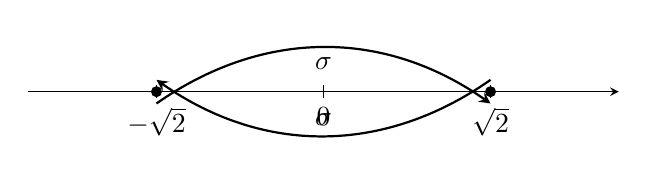
\begin{tikzpicture}[x=1.5cm,>=stealth]
\draw[->] (-2.5,0)--(2.5,0);
\foreach \x/\lab in {-1.414/{-\sqrt2},0/0,1.414/{\sqrt2}}
    \draw (\x,0.08)--(\x,-0.08) node[below] {\(\lab\)};

\fill (1.414,0) circle (2pt);
\fill (-1.414,0) circle (2pt);

\draw[->,thick,bend left=35] (1.414,0.15) to node[above]{\(\sigma\)} (-1.414,0.15);
\draw[->,thick,bend left=35] (-1.414,-0.15) to node[below]{\(\sigma\)} (1.414,-0.15);
\end{tikzpicture}
\end{center}

The field symmetry exchanges the two roots of

\[ x^2-2. \]

This simple idea becomes the foundation of Galois theory.

%%%%%%%%%%%%%%%%%%%%%%%%%%%%%%%%%%%%%%%%%%%%%%%%%%%%%%%%%%%%
\subsection{Finite Fields}
\label{subsec:finite-fields}
%%%%%%%%%%%%%%%%%%%%%%%%%%%%%%%%%%%%%%%%%%%%%%%%%%%%%%%%%%%%

A field containing finitely many elements is called a
\emph{finite field}.

Finite fields are also called \emph{Galois fields}.

A finite field with \(q\) elements is often denoted

\[ \F_q \]

or

\[ GF(q). \]

The notation \(GF(q)\) is read ``G-F of \(q\)'' or ``the Galois field with
\(q\) elements.''

%%%%%%%%%%%%%%%%%%%%%%%%%%%%%%%%%%%%%%%%%%%%%%%%%%%%%%%%%%%%
\subsection{Possible Sizes of Finite Fields}
\label{subsec:finite-field-orders}
%%%%%%%%%%%%%%%%%%%%%%%%%%%%%%%%%%%%%%%%%%%%%%%%%%%%%%%%%%%%

Finite fields do not exist for arbitrary sizes.

\begin{theorem}
Every finite field has
\[ p^n \]
elements for some prime \(p\) and positive integer \(n\).
\end{theorem}

Conversely, for every prime power

\[ q=p^n, \]

there exists a finite field with \(q\) elements, unique up to isomorphism.

Thus finite fields exist with sizes such as

\[ 2,\ 3,\ 4,\ 5,\ 7,\ 8,\ 9,\ 11,\ 13,\ 16,\ldots \]

but not with \(6\), \(10\), \(12\), or other non-prime-power sizes.

%%%%%%%%%%%%%%%%%%%%%%%%%%%%%%%%%%%%%%%%%%%%%%%%%%%%%%%%%%%%
\subsection{Why Finite Fields Have Prime-Power Size}
\label{subsec:finite-fields-prime-power}
%%%%%%%%%%%%%%%%%%%%%%%%%%%%%%%%%%%%%%%%%%%%%%%%%%%%%%%%%%%%

Let \(F\) be a finite field of characteristic \(p\).

Its prime subfield is

\[ \F_p. \]

Therefore \(F\) is a finite-dimensional vector space over \(\F_p\).

Suppose

\[ [F:\F_p]=n. \]

A vector in an \(n\)-dimensional vector space over \(\F_p\) is determined by
\(n\) coordinates, each having \(p\) choices.

Therefore,

\[ |F|=p^n. \]

This is a striking example of linear algebra determining field structure.

%%%%%%%%%%%%%%%%%%%%%%%%%%%%%%%%%%%%%%%%%%%%%%%%%%%%%%%%%%%%
\subsection{Visualizing a Finite Field as a Vector Space}
\label{subsec:finite-field-vector-space}
%%%%%%%%%%%%%%%%%%%%%%%%%%%%%%%%%%%%%%%%%%%%%%%%%%%%%%%%%%%%

For a degree-\(2\) extension of \(\F_p\), elements have the form

\[ a+b\alpha,\qquad a,b\in\F_p. \]

The coefficient choices can be pictured as a \(p\times p\) grid:

\begin{center}
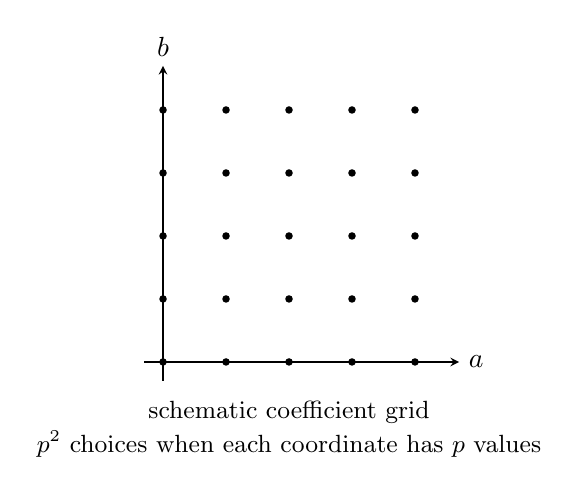
\begin{tikzpicture}[scale=0.8,>=stealth]
\draw[->] (-0.3,0)--(4.7,0) node[right]{\(a\)};
\draw[->] (0,-0.3)--(0,4.7) node[above]{\(b\)};

\foreach \x in {0,...,4}{
    \foreach \y in {0,...,4}{
        \fill (\x,\y) circle (1.7pt);
    }
}

\node at (2,-0.8) {\small schematic coefficient grid};
\node at (2,-1.3) {\small \(p^2\) choices when each coordinate has \(p\) values};
\end{tikzpicture}
\end{center}

The diagram is schematic; the important principle is

\[ p\text{ choices per coordinate}\times n\text{ coordinates}=p^n\text{ vectors}. \]

%%%%%%%%%%%%%%%%%%%%%%%%%%%%%%%%%%%%%%%%%%%%%%%%%%%%%%%%%%%%
\subsection{Constructing \(\F_{p^n}\)}
\label{subsec:constructing-finite-fields}
%%%%%%%%%%%%%%%%%%%%%%%%%%%%%%%%%%%%%%%%%%%%%%%%%%%%%%%%%%%%

Let

\[ f(x)\in\F_p[x] \]

be irreducible of degree \(n\).

Then

\[ \F_p[x]/(f(x)) \]

is a field containing

\[ p^n \]

elements.

This gives a practical construction of finite field extensions.

%%%%%%%%%%%%%%%%%%%%%%%%%%%%%%%%%%%%%%%%%%%%%%%%%%%%%%%%%%%%
\subsection{Example: Constructing a Field with Four Elements}
\label{subsec:field-four-elements}
%%%%%%%%%%%%%%%%%%%%%%%%%%%%%%%%%%%%%%%%%%%%%%%%%%%%%%%%%%%%

Over \(\F_2\), consider

\[ f(x)=x^2+x+1. \]

It has no roots in \(\F_2\), since

\[ f(0)=1,\qquad f(1)=1. \]

Therefore it is irreducible over \(\F_2\).

Construct

\[ \F_2[x]/(x^2+x+1). \]

Let

\[ \alpha=[x]. \]

Then

\[ \alpha^2+\alpha+1=0, \]

so

\[ \alpha^2=\alpha+1 \]

because subtraction and addition coincide in characteristic \(2\).

The field has four elements:

\[ \{0,1,\alpha,\alpha+1\}. \]

%%%%%%%%%%%%%%%%%%%%%%%%%%%%%%%%%%%%%%%%%%%%%%%%%%%%%%%%%%%%
\subsection{Arithmetic in \(\F_4\)}
\label{subsec:arithmetic-f4}
%%%%%%%%%%%%%%%%%%%%%%%%%%%%%%%%%%%%%%%%%%%%%%%%%%%%%%%%%%%%

Using

\[ \alpha^2=\alpha+1, \]

we obtain

\[ \alpha(\alpha+1)=\alpha^2+\alpha=(\alpha+1)+\alpha=1. \]

Thus

\[ \alpha^{-1}=\alpha+1. \]

Similarly,

\[ (\alpha+1)^2=\alpha. \]

The nonzero elements form a cyclic multiplicative group of order \(3\).

%%%%%%%%%%%%%%%%%%%%%%%%%%%%%%%%%%%%%%%%%%%%%%%%%%%%%%%%%%%%
\subsection{Worked Example: Multiplication in \(\F_4\)}
\label{subsec:worked-f4}
%%%%%%%%%%%%%%%%%%%%%%%%%%%%%%%%%%%%%%%%%%%%%%%%%%%%%%%%%%%%

\begin{workedexamplebox}{Multiplication in a Finite Field}

In

\[ \F_4=\F_2(\alpha),\qquad \alpha^2+\alpha+1=0, \]

compute

\[ (\alpha+1)^2. \]

\begin{tabularx}{\textwidth}{@{}>{\raggedright\arraybackslash}p{0.42\textwidth}X@{}}
Expand. & \((\alpha+1)^2=\alpha^2+2\alpha+1\)\\
Use characteristic \(2\). & \(2\alpha=0\)\\
Use \(\alpha^2=\alpha+1\). & \((\alpha+1)^2=(\alpha+1)+1\)\\
Simplify in characteristic \(2\). & \((\alpha+1)^2=\alpha\)
\end{tabularx}

\begin{answerbox}
\[ (\alpha+1)^2=\alpha. \]
\end{answerbox}
\end{workedexamplebox}

%%%%%%%%%%%%%%%%%%%%%%%%%%%%%%%%%%%%%%%%%%%%%%%%%%%%%%%%%%%%
\subsection{The Frobenius Map}
\label{subsec:frobenius-map}
%%%%%%%%%%%%%%%%%%%%%%%%%%%%%%%%%%%%%%%%%%%%%%%%%%%%%%%%%%%%

Fields of positive characteristic possess an important natural map.

\begin{definitionbox}{Frobenius Map}
If \(F\) has characteristic \(p\), the \emph{Frobenius map} is
\[ \Phi:F\to F,\qquad \Phi(a)=a^p. \]
\end{definitionbox}

The symbol

\[ \Phi \]

is uppercase Greek \emph{Phi}, commonly pronounced ``fie'' or ``fee.''

The map is named after Ferdinand Georg Frobenius.

%%%%%%%%%%%%%%%%%%%%%%%%%%%%%%%%%%%%%%%%%%%%%%%%%%%%%%%%%%%%
\subsection{Why Frobenius Preserves Addition}
\label{subsec:frobenius-addition}
%%%%%%%%%%%%%%%%%%%%%%%%%%%%%%%%%%%%%%%%%%%%%%%%%%%%%%%%%%%%

In characteristic \(p\),

\[ (a+b)^p=a^p+b^p. \]

The intermediate binomial coefficients

\[ \binom{p}{k} \]

are divisible by \(p\) for

\[ 1\leq k\leq p-1. \]

Therefore they become zero in characteristic \(p\).

Hence

\[ \Phi(a+b)=\Phi(a)+\Phi(b). \]

Also,

\[ \Phi(ab)=a^pb^p=\Phi(a)\Phi(b). \]

Thus Frobenius is a field homomorphism.

%%%%%%%%%%%%%%%%%%%%%%%%%%%%%%%%%%%%%%%%%%%%%%%%%%%%%%%%%%%%
\subsection{Frobenius on Finite Fields}
\label{subsec:frobenius-finite-fields}
%%%%%%%%%%%%%%%%%%%%%%%%%%%%%%%%%%%%%%%%%%%%%%%%%%%%%%%%%%%%

Because every field homomorphism is injective, Frobenius is injective.

On a finite field, every injective map from the field to itself is also
surjective.

Therefore Frobenius is an automorphism of every finite field.

For

\[ \F_p, \]

Fermat's theorem gives

\[ a^p=a \]

for every \(a\in\F_p\).

Thus Frobenius acts as the identity on the prime field.

%%%%%%%%%%%%%%%%%%%%%%%%%%%%%%%%%%%%%%%%%%%%%%%%%%%%%%%%%%%%
\subsection{Roots and Field Extensions}
\label{subsec:roots-field-extensions}
%%%%%%%%%%%%%%%%%%%%%%%%%%%%%%%%%%%%%%%%%%%%%%%%%%%%%%%%%%%%

Field theory changes the question

\begin{center}
``Does this polynomial have a root?''
\end{center}

into the more structural question

\begin{center}
``What is the smallest field in which this polynomial has its roots?''
\end{center}

For example,

\[ x^2-2 \]

has no root in \(\Q\), but it has roots in

\[ \Q(\sqrt2). \]

Likewise,

\[ x^2+1 \]

has no root in \(\R\), but it has roots in

\[ \C. \]

%%%%%%%%%%%%%%%%%%%%%%%%%%%%%%%%%%%%%%%%%%%%%%%%%%%%%%%%%%%%
\subsection{A Root-Extension Flow Diagram}
\label{subsec:root-extension-flow}
%%%%%%%%%%%%%%%%%%%%%%%%%%%%%%%%%%%%%%%%%%%%%%%%%%%%%%%%%%%%

\begin{center}
\begin{tikzpicture}[
    node distance=11mm,
    box/.style={draw,rounded corners,align=center,inner sep=5pt,font=\small},
    >=stealth
]
\node[box] (poly) {Polynomial \(f(x)\in K[x]\)};
\node[box,below=of poly] (root) {Does \(f\) have all roots in \(K\)?};
\node[box,below left=of root] (yes) {Yes\\factor in \(K[x]\)};
\node[box,below right=of root] (no) {No\\adjoin missing roots};
\node[box,below=of no] (ext) {Extension field \(L\)};
\node[box,below=of ext] (split) {Splitting field};

\draw[->] (poly)--(root);
\draw[->] (root)--node[left]{yes}(yes);
\draw[->] (root)--node[right]{no}(no);
\draw[->] (no)--(ext);
\draw[->] (ext)--(split);
\end{tikzpicture}
\end{center}

%%%%%%%%%%%%%%%%%%%%%%%%%%%%%%%%%%%%%%%%%%%%%%%%%%%%%%%%%%%%
\subsection{Common Errors in Field Theory}
\label{subsec:common-field-errors}
%%%%%%%%%%%%%%%%%%%%%%%%%%%%%%%%%%%%%%%%%%%%%%%%%%%%%%%%%%%%

\subsubsection{Assuming Every Integral Domain Is a Field}

Every field is an integral domain, but the converse is false.

For example,

\[ \Z \]

is an integral domain but not a field.

%%%%%%%%%%%%%%%%%%%%%%%%%%%%%%%%%%%%%%%%%%%%%%%%%%%%%%%%%%%%
\subsubsection{Assuming Every \(\Z_n\) Is a Field}

The ring

\[ \Z_n \]

is a field precisely when \(n\) is prime.

For example,

\[ \Z_7 \]

is a field, while

\[ \Z_8 \]

is not.

%%%%%%%%%%%%%%%%%%%%%%%%%%%%%%%%%%%%%%%%%%%%%%%%%%%%%%%%%%%%
\subsubsection{Confusing \(L/K\) with Division}

The notation

\[ L/K \]

for a field extension does not mean a quotient or numerical division.

It means that \(K\) is a subfield of \(L\).

%%%%%%%%%%%%%%%%%%%%%%%%%%%%%%%%%%%%%%%%%%%%%%%%%%%%%%%%%%%%
\subsubsection{Confusing \(K[\alpha]\) and \(K(\alpha)\)}

The notation

\[ K[\alpha] \]

means the smallest subring containing \(K\) and \(\alpha\).

The notation

\[ K(\alpha) \]

means the smallest subfield containing them.

If \(\alpha\) is algebraic over a field \(K\), then

\[ K[\alpha]=K(\alpha). \]

For transcendental \(\alpha\), these structures generally differ.

%%%%%%%%%%%%%%%%%%%%%%%%%%%%%%%%%%%%%%%%%%%%%%%%%%%%%%%%%%%%
\subsubsection{Assuming Every Extension Is Finite}

An extension may have infinite dimension.

Thus

\[ [L:K] \]

need not be finite.

%%%%%%%%%%%%%%%%%%%%%%%%%%%%%%%%%%%%%%%%%%%%%%%%%%%%%%%%%%%%
\subsubsection{Assuming Algebraic Means Rational}

An algebraic number over \(\Q\) need not be rational.

For example,

\[ \sqrt2 \]

is irrational but algebraic.

%%%%%%%%%%%%%%%%%%%%%%%%%%%%%%%%%%%%%%%%%%%%%%%%%%%%%%%%%%%%
\subsubsection{Assuming Irrational Means Transcendental}

An irrational number may be algebraic.

For example,

\[ \sqrt2,\qquad\sqrt3,\qquad\sqrt[3]{5} \]

are irrational algebraic numbers.

Transcendence is a stronger condition.

%%%%%%%%%%%%%%%%%%%%%%%%%%%%%%%%%%%%%%%%%%%%%%%%%%%%%%%%%%%%
\subsubsection{Using a Polynomial That Is Not Minimal}

A polynomial satisfied by \(\alpha\) need not be its minimal polynomial.

For example, \(\sqrt2\) satisfies

\[ x^4-4=0, \]

but its minimal polynomial over \(\Q\) is

\[ x^2-2. \]

%%%%%%%%%%%%%%%%%%%%%%%%%%%%%%%%%%%%%%%%%%%%%%%%%%%%%%%%%%%%
\subsubsection{Forgetting the Base Field}

Algebraicity and irreducibility depend on the base field.

For example,

\[ x^2-2 \]

is irreducible over \(\Q\), but over \(\R\),

\[ x^2-2=(x-\sqrt2)(x+\sqrt2). \]

Thus the phrase ``irreducible polynomial'' is incomplete unless the
coefficient field is understood.

%%%%%%%%%%%%%%%%%%%%%%%%%%%%%%%%%%%%%%%%%%%%%%%%%%%%%%%%%%%%
\subsection{Applications of Field Theory}
\label{subsec:field-theory-applications}
%%%%%%%%%%%%%%%%%%%%%%%%%%%%%%%%%%%%%%%%%%%%%%%%%%%%%%%%%%%%

\begin{applicationbox}
\textbf{Linear Algebra.}
Vector spaces require a field of scalars. Changing the scalar field can change
dimension, independence, eigenvalues, and diagonalizability.

\medskip

\textbf{Polynomial Equations.}
Field extensions provide systematic ways to adjoin roots and construct
splitting fields.

\medskip

\textbf{Galois Theory.}
Automorphisms of field extensions encode symmetries among polynomial roots
and connect field structure with group theory.

\medskip

\textbf{Number Theory.}
Algebraic number fields extend \(\Q\) by adjoining algebraic numbers and form
a central setting for algebraic number theory.

\medskip

\textbf{Geometry.}
Fields determine the coordinate systems over which algebraic and projective
geometric objects are studied.

\medskip

\textbf{Finite Geometry.}
Finite fields provide coordinate systems for finite projective and affine
geometries.

\medskip

\textbf{Coding Theory.}
Error-correcting codes are frequently constructed using vector spaces and
polynomials over finite fields.

\medskip

\textbf{Cryptography.}
Finite fields are fundamental in modern cryptographic systems, including
elliptic-curve cryptography.

\medskip

\textbf{Computer Science.}
Finite-field arithmetic appears in data storage, communication protocols,
checksums, and symbolic computation.
\end{applicationbox}

%%%%%%%%%%%%%%%%%%%%%%%%%%%%%%%%%%%%%%%%%%%%%%%%%%%%%%%%%%%%
\subsection{Structural Map of Field Theory}
\label{subsec:field-theory-structure-map}
%%%%%%%%%%%%%%%%%%%%%%%%%%%%%%%%%%%%%%%%%%%%%%%%%%%%%%%%%%%%

\begin{center}
\begin{tikzpicture}[
    node distance=10mm and 14mm,
    box/.style={draw,rounded corners,align=center,inner sep=4pt,font=\small},
    >=stealth
]
\node[box] (field) {Field};
\node[box,below left=of field] (char) {Characteristic};
\node[box,below right=of field] (ext) {Extensions};

\node[box,below=of char] (prime) {Prime subfield};
\node[box,below left=of ext] (alg) {Algebraic};
\node[box,below right=of ext] (trans) {Transcendental};

\node[box,below=of alg] (minimal) {Minimal polynomials};
\node[box,below=of trans] (degree) {Extension degree};

\node[box,below=of minimal] (split) {Splitting fields};
\node[box,below=of degree] (finite) {Finite fields};

\node[box,below right=of split] (auto) {Field automorphisms};
\node[box,below=of auto] (galois) {Galois theory};

\draw[->] (field)--(char);
\draw[->] (field)--(ext);
\draw[->] (char)--(prime);
\draw[->] (ext)--(alg);
\draw[->] (ext)--(trans);
\draw[->] (alg)--(minimal);
\draw[->] (trans)--(degree);
\draw[->] (minimal)--(split);
\draw[->] (degree)--(finite);
\draw[->] (split)--(auto);
\draw[->] (finite)--(auto);
\draw[->] (auto)--(galois);
\end{tikzpicture}
\end{center}

%%%%%%%%%%%%%%%%%%%%%%%%%%%%%%%%%%%%%%%%%%%%%%%%%%%%%%%%%%%%
\subsection{Exercises}
\label{subsec:field-theory-exercises}
%%%%%%%%%%%%%%%%%%%%%%%%%%%%%%%%%%%%%%%%%%%%%%%%%%%%%%%%%%%%

\begin{exercise}[1]
Explain why \(\Q\) is a field.
\end{exercise}

\begin{exercise}[1]
Explain why \(\Z\) is not a field.
\end{exercise}

\begin{exercise}[1]
Determine whether \(\Z_5\) is a field.
\end{exercise}

\begin{exercise}[1]
Determine whether \(\Z_9\) is a field.
\end{exercise}

\begin{exercise}[1]
Find the multiplicative inverse of every nonzero element of \(\F_7\).
\end{exercise}

\begin{exercise}[2]
Solve
\[ [4]_7x=[3]_7 \]
in \(\F_7\).
\end{exercise}

\begin{exercise}[2]
Prove that every field is an integral domain.
\end{exercise}

\begin{exercise}[2]
Prove that a finite integral domain is a field.
\end{exercise}

\begin{exercise}[1]
Find
\[ \operatorname{char}(\Q),\qquad\operatorname{char}(\F_5),\qquad\operatorname{char}(\C). \]
\end{exercise}

\begin{exercise}[2]
Explain why a field cannot have characteristic \(6\).
\end{exercise}

\begin{exercise}[2]
Determine the prime subfield of \(\R\).
\end{exercise}

\begin{exercise}[2]
Determine the prime subfield of a field of characteristic \(11\).
\end{exercise}

\begin{exercise}[2]
Use the subfield test to verify
\[ \Q\subseteq\R. \]
\end{exercise}

\begin{exercise}[1]
Explain what the notation
\[ \C/\R \]
means.
\end{exercise}

\begin{exercise}[1]
Find
\[ [\C:\R]. \]
\end{exercise}

\begin{exercise}[2]
Give a basis for \(\C\) as a vector space over \(\R\).
\end{exercise}

\begin{exercise}[2]
Show that
\[ \Q(\sqrt5)=\{a+b\sqrt5:a,b\in\Q\}. \]
\end{exercise}

\begin{exercise}[2]
Find
\[ [\Q(\sqrt5):\Q]. \]
\end{exercise}

\begin{exercise}[2]
Find the inverse of
\[ 3+2\sqrt2 \]
inside \(\Q(\sqrt2)\).
\end{exercise}

\begin{exercise}[2]
Find the minimal polynomial of \(\sqrt5\) over \(\Q\).
\end{exercise}

\begin{exercise}[2]
Find the minimal polynomial of \(i\) over \(\R\).
\end{exercise}

\begin{exercise}[2]
Find the minimal polynomial of \(\sqrt[3]{2}\) over \(\Q\).
\end{exercise}

\begin{exercise}[2]
Determine
\[ [\Q(\sqrt[3]{2}):\Q]. \]
\end{exercise}

\begin{exercise}[3]
Prove that if \(\alpha\) is algebraic over \(K\) and its minimal polynomial has
degree \(n\), then
\[ \{1,\alpha,\ldots,\alpha^{n-1}\} \]
is a basis for \(K(\alpha)\) over \(K\).
\end{exercise}

\begin{exercise}[2]
Suppose
\[ K\subseteq L\subseteq M \]
with
\[ [L:K]=5,\qquad[M:L]=3. \]
Find \([M:K]\).
\end{exercise}

\begin{exercise}[3]
Suppose
\[ [M:K]=15,\qquad[L:K]=5. \]
If \(K\subseteq L\subseteq M\), determine \([M:L]\).
\end{exercise}

\begin{exercise}[3]
Prove that every finite extension is algebraic.
\end{exercise}

\begin{exercise}[2]
Explain why \(\pi\) being transcendental over \(\Q\) implies that it is not
algebraic over \(\Q\).
\end{exercise}

\begin{exercise}[2]
Explain why \(\sqrt2\) is irrational but algebraic.
\end{exercise}

\begin{exercise}[2]
Construct
\[ \Q(\sqrt3) \]
as a quotient of a polynomial ring.
\end{exercise}

\begin{exercise}[2]
Explain why
\[ \R[x]/(x^2+1)\cong\C. \]
\end{exercise}

\begin{exercise}[2]
Find the splitting field of
\[ x^2-5 \]
over \(\Q\).
\end{exercise}

\begin{exercise}[2]
Find the splitting field of
\[ x^2+4 \]
over \(\R\).
\end{exercise}

\begin{exercise}[2]
Does
\[ x^2+1 \]
split over \(\Q\)? Over \(\R\)? Over \(\C\)?
\end{exercise}

\begin{exercise}[2]
Explain what it means for a field to be algebraically closed.
\end{exercise}

\begin{exercise}[2]
Explain why \(\R\) is not algebraically closed.
\end{exercise}

\begin{exercise}[2]
Explain why every field homomorphism is injective.
\end{exercise}

\begin{exercise}[2]
Verify that
\[ \sigma(a+b\sqrt2)=a-b\sqrt2 \]
defines an automorphism of \(\Q(\sqrt2)\).
\end{exercise}

\begin{exercise}[2]
Determine all possible sizes of finite fields less than \(20\).
\end{exercise}

\begin{exercise}[2]
Explain why no field with exactly \(6\) elements exists.
\end{exercise}

\begin{exercise}[2]
Explain why a field with \(8\) elements can exist.
\end{exercise}

\begin{exercise}[3]
Prove that every finite field has prime-power order.
\end{exercise}

\begin{exercise}[2]
Show that
\[ x^2+x+1 \]
is irreducible over \(\F_2\).
\end{exercise}

\begin{exercise}[2]
List the four elements of
\[ \F_2[x]/(x^2+x+1). \]
\end{exercise}

\begin{exercise}[2]
Using
\[ \alpha^2+\alpha+1=0, \]
compute
\[ \alpha^3. \]
\end{exercise}

\begin{exercise}[3]
Construct the multiplication table for
\[ \F_4=\{0,1,\alpha,\alpha+1\}. \]
\end{exercise}

\begin{exercise}[3]
Show that the nonzero elements of \(\F_4\) form a cyclic group.
\end{exercise}

\begin{exercise}[3]
Let \(F\) have characteristic \(p\). Prove
\[ (a+b)^p=a^p+b^p. \]
\end{exercise}

\begin{exercise}[3]
Show that the Frobenius map
\[ \Phi(a)=a^p \]
is a field homomorphism.
\end{exercise}

\begin{exercise}[3]
Explain why Frobenius is an automorphism on every finite field.
\end{exercise}

\begin{exercise}[3]
Create a field-extension diagram containing
\[ \Q,\qquad\Q(\sqrt2),\qquad\R,\qquad\C \]
and indicate all valid inclusions.
\end{exercise}

%%%%%%%%%%%%%%%%%%%%%%%%%%%%%%%%%%%%%%%%%%%%%%%%%%%%%%%%%%%%
\subsection{Section Connections}
\label{subsec:field-theory-connections}
%%%%%%%%%%%%%%%%%%%%%%%%%%%%%%%%%%%%%%%%%%%%%%%%%%%%%%%%%%%%

\chapterconnection{
Field theory provides the canonical theory of algebraic systems in which
addition, subtraction, multiplication, and division by nonzero elements are
available. It also provides the scalar systems underlying vector spaces from
\cref{sec:linear-algebra}. The theory of field extensions connects polynomial
rings from \cref{sec:ring-theory} with roots of equations, while field
automorphisms connect these extensions back to the symmetry structures of
\cref{sec:group-theory}. These ideas lead directly to Galois theory, where
groups of field automorphisms are used to study polynomial equations.
Finite fields later reappear in number theory, combinatorics, coding theory,
finite geometry, and cryptography.
}

%%%%%%%%%%%%%%%%%%%%%%%%%%%%%%%%%%%%%%%%%%%%%%%%%%%%%%%%%%%%
% SECTION SOURCE TRACKING
%%%%%%%%%%%%%%%%%%%%%%%%%%%%%%%%%%%%%%%%%%%%%%%%%%%%%%%%%%%%

%------------------------------------------------------------
% 1.6 Field Theory
%------------------------------------------------------------
%
% Sources:
%   - Thomas W. Judson, Abstract Algebra: Theory and Applications.
%     Key: judson2025abstractalgebra
%
% Used for:
%   - fields and subfields;
%   - field characteristic and prime subfields;
%   - field extensions;
%   - algebraic and transcendental elements;
%   - minimal polynomials;
%   - extension degrees and the Tower Law;
%   - polynomial quotient constructions;
%   - splitting fields and algebraic closures;
%   - field embeddings and automorphisms;
%   - finite-field foundations and standard examples.
%
% Notes:
%   - Basic ring structure is treated canonically in Section 1.5.
%   - Vector-space foundations are treated canonically in Section 1.2.
%   - This section develops field extensions sufficiently to support
%     Galois theory without duplicating the detailed Galois correspondence.
%   - Detailed finite-field applications may later be cross-referenced from
%     number theory, coding theory, combinatorics, and cryptography.
%   - Advanced field-theoretic topics such as separability, normality,
%     purely inseparable extensions, transcendence bases, and detailed
%     algebraic closure theory are introduced only as needed here and may
%     be developed further in specialized sections.
%   - Visualizations and exposition are independently developed for this text.
%
\nocite{judson2025abstractalgebra}